\documentclass[a4paper]{article} 

\usepackage{graphicx}
\graphicspath{ {./images/} }
\usepackage{wrapfig}

\addtolength{\hoffset}{-2.25cm}
\addtolength{\textwidth}{4.5cm}
\addtolength{\voffset}{-3.25cm}
\addtolength{\textheight}{5cm}
\setlength{\parskip}{0pt}
\setlength{\parindent}{0in}

%----------------------------------------------------------------------------------------
%	PACKAGES AND OTHER DOCUMENT CONFIGURATIONS
%----------------------------------------------------------------------------------------

\usepackage{blindtext} % Package to generate dummy text
\usepackage{charter} % Use the Charter font
\usepackage[utf8]{inputenc} % Use UTF-8 encoding
\usepackage{microtype} % Slightly tweak font spacing for aesthetics
\usepackage[english, ngerman]{babel} % Language hyphenation and typographical rules
\usepackage{amsthm, amsmath, amssymb} % Mathematical typesetting
\usepackage{float} % Improved interface for floating objects
\usepackage[final, colorlinks = true, 
            linkcolor = black, 
            citecolor = black]{hyperref} % For hyperlinks in the PDF
\usepackage{graphicx, multicol} % Enhanced support for graphics
\usepackage{xcolor} % Driver-independent color extensions
\usepackage{marvosym, wasysym} % More symbols
\usepackage{rotating} % Rotation tools
\usepackage{censor} % Facilities for controlling restricted text
\usepackage{listings, style/lstlisting} % Environment for non-formatted code, !uses style file!
\usepackage{pseudocode} % Environment for specifying algorithms in a natural way
\usepackage{style/avm} % Environment for f-structures, !uses style file!
\usepackage{booktabs} % Enhances quality of tables
\usepackage{tikz-qtree} % Easy tree drawing tool
\tikzset{every tree node/.style={align=center,anchor=north},
         level distance=2cm} % Configuration for q-trees
\usepackage{style/btree} % Configuration for b-trees and b+-trees, !uses style file!
\usepackage[backend=biber,style=numeric,
            sorting=nyt]{biblatex} % Complete reimplementation of bibliographic facilities
\addbibresource{ecl.bib}
\usepackage{csquotes} % Context sensitive quotation facilities
\usepackage[yyyymmdd]{datetime} % Uses YEAR-MONTH-DAY format for dates
\renewcommand{\dateseparator}{-} % Sets dateseparator to '-'
\usepackage{fancyhdr} % Headers and footers
\pagestyle{fancy} % All pages have headers and footers
\fancyhead{}\renewcommand{\headrulewidth}{0pt} % Blank out the default header
\fancyfoot[L]{} % Custom footer text
\fancyfoot[C]{} % Custom footer text
\fancyfoot[R]{\thepage} % Custom footer text
\newcommand{\note}[1]{\marginpar{\scriptsize \textcolor{red}{#1}}} % Enables comments in red on margin

%----------------------------------------------------------------------------------------

\begin{document}

%-------------------------------
%	TITLE SECTION
%-------------------------------

\fancyhead[C]{}
\hrule \medskip % Upper rule
\begin{minipage}{0.24\textwidth} 
\raggedright
\footnotesize
Quentin Le Roux \hfill
\end{minipage}
\begin{minipage}{0.5\textwidth} 
\centering 
Seminar 1 -- Histopathology -- 1-page Summary
\end{minipage}
\begin{minipage}{0.245\textwidth} 
\raggedleft
\today
\end{minipage}
\hrule 
\bigskip

%-------------------------------
%	CONTENTS
%-------------------------------

The seminar covered an \textbf{introduction to machine learning for histopathology}, presented by Paul Tourniaire as part of the 3iA Côte d'Azur Institute. 
%, a newly created expertise center that aims to create an innovative ecosystem with a local, national and international reach.
\\\\
Histopathology is the golden standard of cancer treatment, and pathologists in the French multi-disciplinary framework of diagnosis (i.e. RCP) play a key role in helping diagnose cancer (e.g. tumor size, metastasis, nodes) and chart a treatment procedure. The question is: 

\begin{center}
\textit{Can AI help pathologists diagnose cancer and assign the best treatment}?
\end{center}

\section{Research's Goal}
The research (by P. Tourniaire, H. Delingette, M. Ilié, P. Hofman, and N. Ayache) aims to develop an \textbf{AI-based selection of imaging and biological merkers} that have a predictive value in terms of therapy response for Non Small Cell Lung Cancers (abbr. NSCLC). 

It resulted in a multimodal model (taking data from three categories: HES Whole Slice Images (WSI), IHC slides, and bionomics) to predict immunotherapy response first, then possibly lead to the discovery of new predictive biomarkers for treatment success

\section{Data Available and Usage}

\begin{wrapfigure}{r}{0.25\textwidth} %this figure will be at the right
    \centering
    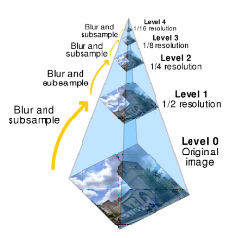
\includegraphics[width=0.2\textwidth]{pyramid}\\
    {\scriptsize Figure 1: Pyramidal Image Structure}
\end{wrapfigure}

In histopathology, data is obtained via biopsy and resection. Tissues are sliced and stained to obtain digitized slides. Histopathology works with a digitized file format called a pyramidal file (see figure 1).

That format offers varying magnifications in order to perform different level of analyses. To help, researchers have access to general Python tools for computer vision (e.g. scikit-learn, PIL) and dedicated tools for WSI (e.g. openslide, pyvips).

\section{Issues and Challenges}

WSI are large and cannot be processed at once. A tiling approach is almost always necessary. Due to this (different magnifications and tiling), the learning approach is a type of multiple instance learning (MIL).

All together, WSI are stained with color agents (e.g. hematoxylin) which are not normalized and lead to colour discrepancies -- another issue. Meanwhile many types of artefacts have to be accounted for (e.g. folds, tears). A strong pre-processing phase is necessary.

\section{Pipeline and Models Covered}

Slides are pre-processed using multiple, successive methods (see figure 2). More complex combination of image filters and classifiers can be applied (e.g. HistoQC). Once images are pre-processed, they can be fed into a model, three of which the presented research showcased.\\
\begin{wrapfigure}{r}{0.7\linewidth}
\centering
\fbox{\parbox[t]{5em}{{\scriptsize First task\\\\Grayscaling\\Thresholding}}}%
\raisebox{-4ex}{$\to$}%
\fbox{\parbox[t]{8.5em}{{\scriptsize Second Task\\\\filter out noisy elements}}}%
\raisebox{-4ex}{$\to$}%
\fbox{\parbox[t]{4.5em}{{\scriptsize Third Task\\\\Tiling}}}
\raisebox{-4ex}{$\to$}%
\fbox{\parbox[t]{8em}{{\scriptsize Fourth Task\\\\Staining Normalization (macenko method)}}}
\\{\scriptsize Figure 2: Pre-processing Pipeline}
\end{wrapfigure}

Three models were presented: CLAM (ResNet50 performing feature extraction followed by Multi-Class Attention Branches that yields an attention score), MIL+RNN (classifier RNN that outputs slide targets), CHOWDER (Uses local descriptors and a CNN to output classifier predictions).

The performance is checked via a Area under the Curve (AuC) metric using mean-pooling as a baseline.
\section{Conclusion}
Computational histopathology has now reached human-comparable results on cancer related tissues in many different tasks such as tumour classification, or survival prediction.
\end{document}

%doc by Quentin Le Roux